We consider a system consisting of two phases, separated by a sharp interface $\Sigma(t)$ which evolves over time. 
Each phase subdomain is denoted $\Omega_1(t)$ and $\Omega_2(t)$ for the continuous phase ($1$) and the dispersed phase ($2$) respectively (see \ref{fig:Scheme}). 
The mathematical and physical definition of $\Sigma(t)$ is by no means straightforward, therefore, the interested reader is refereed to \cite{bothe2022sharp} to have a deeper understanding of sharp interface modeling. 
The entire domain, denoted as $\Omega$, is defined as the union of $\Omega_1$, $\Omega_2$, and $\Sigma$.
To track the position of the phase indexed $k$, we introduce the phase indicator function, 
\begin{equation}
    \chi_k(\textbf{y},t) =  \left\{
      \begin{tabular}{cc}
        $1 \;\text{if} \;\textbf{y} \in \Omega_k(t)$\\
        $0 \;\text{if} \;\textbf{y} \notin \Omega_k(t)$
      \end{tabular}
      \right.
      \text{for $k = 1,2$}
      \label{eq:PIF}
\end{equation}
which is null everywhere except inside the phase $k$. 
In the following, we omit the time and position arguments of $\chi_k$. 
\begin{figure}[h!]
    \centering
    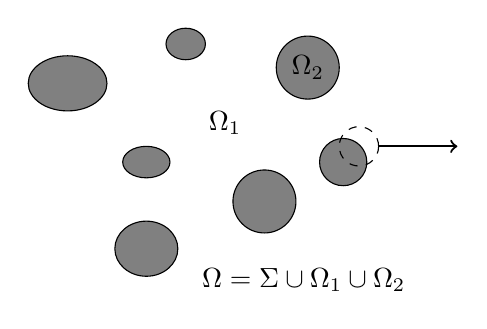
\begin{tikzpicture}
        \foreach \x/\y/\ra/\r in {
        1/3/0.2/0.25,
        2.55/2.7/0.4/0.4,
        0.5/0.4/0.35/0.4,
        2/1/0.4/0.4,
        3/1.5/0.3/0.3,
        0.5/1.5/0.2/0.3,
        -0.5/2.5/0.35/0.5}{
            \draw[fill=gray](\x,\y) ellipse(\r cm and \ra cm);
        }
        \draw[dashed](3.2,1.7)circle(0.25);
        % \draw[thick,->](3.2,1.7)++(0.1767,0.1767)--++(0.4,0.4)--++(1,0);
        \draw[thick,->](3.2,1.7)++(0.25,0)--++(1,0);
        \draw(2.55,2.7)node{$\Omega_2$};
        \draw(1.5,2)node{$\Omega_1$};
        \draw(2.5,0)node{$\Omega = \Sigma \cup \Omega_1 \cup \Omega_2$};
        % \draw(2.5,-1)node{$\Sigma = \sum_\alpha \Sigma_\alpha$};
        % \draw(2.5,-0.5)node{$\Omega_2 = \sum_\alpha \Omega_\alpha$};
    \end{tikzpicture}
    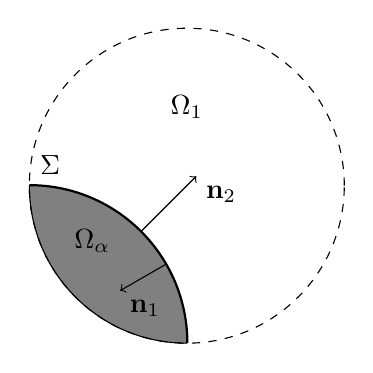
\begin{tikzpicture}%[scale = 0.9]
        \draw[very thick](0:2)arc(0:90:2)node[above right]{$\Sigma$};
        \draw[fill=gray](0:2)arc(0:90:2)arc(180:270:2);
        \draw[dashed](2,2)circle(2);
        \draw[->](1.42,1.42)--++(0.7,0.7)node[below right]{$\textbf{n}_2$};
        \draw[->](1.73,1)--++(-0.577,-0.333)node[below right]{$\textbf{n}_1$};
        \draw(2,3)node{$\Omega_1$};
        \draw(0.8,1.3)node{$\Omega_\alpha$};
    \end{tikzpicture}
    \caption{Domain definitions and scheme of the topology of dispersed two-phase flows.}
    \label{fig:Scheme}
\end{figure}

\subsection{Topological equations}
Using the distribution formalism, one may show that the transport equation of $\chi_k$ reads\citep{drew1983mathematical} 
\begin{equation}
    \pddt \chi_k
    + \textbf{u}_I \cdot \nablabh \chi_k
    = 0,
    \label{eq:dt_chi_k}
\end{equation}
where $\textbf{u}_I$ is the velocity of the interface $\Sigma(t)$.
Additionally, it can be shown  \citep{drew1983mathematical} that,
\begin{equation}
    \nablabh \chi_k
    = - \delta_I \textbf{n}_k
    \label{eq:grad_chi_k}
\end{equation}
where we introduced the interface indicator function defined as $\delta_I = \delta(\textbf{y}-\textbf{y}_I)$ where $\delta$ is the Dirac-delta function and $\textbf{y}_I$ the position of the interface. 
Furthermore, we introduced $\textbf{n}_k$ as being the outward normal vector associated with the domain $\Omega_k$ (see \ref{fig:Scheme}).
To describe the evolution of $\delta_I$ we take the gradient of \ref{eq:dt_chi_k} which yields \citep{morel2015mathematical},
\begin{equation}
    \pddt \delta_I
    + \nablabh \cdot \left[(\textbf{u}_I\cdot\textbf{n})\textbf{n} \delta_I\right]
    = \delta_I (\textbf{u}_I\cdot\textbf{n})(\nablabh \cdot\textbf{n}),
\end{equation}
where we did not specify the index of \textbf{n} since it appears twice in all terms of the equation. 
As pointed out by \citet{morel2007surface}, it is more convenient to rewrite this equation under the following form,
\begin{equation}
    \pddt \delta_I
    + \nablabh \cdot (\delta_I \textbf{u}_I)
    = \delta_I \nablabhI \cdot \textbf{u}_I,
    \label{eq:dt_delta_I}
\end{equation}
where we introduced the surface divergence operator defined as $\nablabhI \cdot ()= (\textbf{I}-\textbf{nn})\cdot \nablabh \cdot ()$, which correspond to the divergence operator projected on $\Sigma(t)$. 
Throughout this work we use the subscript  $_{||}$ to indicate the projection of a quantity onto the plane tangential to the surface $\Sigma(t)$. 
Specifically, for an arbitrary quantity $\textbf{f}$ defined on $\Sigma(t)$, we denote its tangential projection as $\textbf{f}_{||} = (\textbf{I}-\textbf{nn})\cdot \textbf{f}$. 
We also employ the subscript $_I$ to indicate any quantity inherently defined on the interface. 
Lastly, we derive an expression for the gradient of $\delta_I$ by taking the gradient of \ref{eq:grad_chi_k}, resulting in,
\begin{equation}
    \nablabh\delta_I 
    = \textbf{n} \cdot \nablabh (\textbf{n} \delta_I).
    \label{eq:grad_delta_I}
\end{equation}
Then, \ref{eq:dt_chi_k}, \ref{eq:dt_delta_I}, \ref{eq:grad_delta_I} and \ref{eq:grad_chi_k} are commonly referred to as the topological equations for two-phase flows.

\subsection{Local conservation equations}

Let $f_k(\textbf{y},t)$ denote a volumetric quantity of arbitrary tensorial order defined in $\Omega_k(t)$.
Likewise, let $f_I(\textbf{y}_I,I)$ represent an arbitrary surface property defined on $\Sigma(t)$.
Using the strategy outlined in \citep{bothe2022sharp,morel2015mathematical,slattery2007interfacial}, we can derive the local conservation equations for both $f_k(\textbf{y},t)$ and $f_I(\textbf{y}_I,t)$.
They read,  
\begin{align}
    \label{eq:dt_f_k}
    \pddt f_k
    &= \nablabh \cdot \left(
        \mathbf{\Phi}_k
        - f_k\textbf{u}_k
        \right)
    + \textbf{S}_k
    & \text{ in } \Omega_k(t),&\\
    \pddt f_I  
    &= 
    \nablabhI \cdot (\mathbf{\Phi}_{I||} - f_I \textbf{u}_I)
    + \textbf{S}_I
    - \Jump{
        f_k (\textbf{u}_I - \textbf{u}_k)
        + \mathbf{\Phi}_k
     } 
    & \text{ on } \Sigma(t),&
    \label{eq:dt_f_I}
\end{align}
for respectively, $f_k$ and $f_I$.
The tensors $\mathbf{\Phi}_k$ and $\mathbf{\Phi}_{I||}$ represent the diffusive fluxes corresponding to $f_k$ and $f_I$. 
Notice that $\mathbf{\Phi}_{I||}$ carries the $_{||}$ subscript which implies that only the tangential projection of this tensor remain in the surface balance equation. 
The demonstration can be shown in \citet[Chapter 2]{slattery2007interfacial} for the momentum equation. 
Similarly, $\textbf{S}_k$ and $\textbf{S}_I$ represent the source terms for $f_k$ and $f_I$ respectively.
Lastly, $\textbf{u}_k$ corresponds to the velocity field defined in $\Omega_k(t)$, while $\textbf{u}_I$ corresponds to the velocity field defined on $\Sigma(t)$.
In \ref{eq:dt_f_I} we also introduced the notation $\Jump{\ldots}$, which is defined as $\Jump{\ldots} = \sum_{k=1}^2 [\ldots] \cdot \textbf{n}_k$.
This term account for the discontinuity of the flux $\left[f_k (\textbf{u}_I - \textbf{u}_k)+ \mathbf{\Phi}_k\right]\cdot\textbf{n}_k$ in each phases across the interfaces.
\tb{introduce the jump as the lim at each interface, look in math book too}

For the purpose of clarity, we will now consider the specific case of volumetric and surface momentum conservation without mass transfer.
Within phase $k$, we define $f_k$ as the product of density $\rho_k$ and velocity $\textbf{u}_k$, such that $f_k = \rho_k \textbf{u}_k$ is the momentum within $\Omega_k$.
Furthermore, if we assume that the only body force acting on the system is the acceleration of gravity, denoted as $\textbf{g}$, then the source term $\textbf{S}_k$ can be expressed as $\textbf{S}_k = \rho_k \textbf{g}$.
The, diffusive flux $\mathbf{\Phi}_k$ is the stress tensor, denoted as $\textbf{T}_k$ in this study. 
Substituting these terms into \ref{eq:dt_f_k} yields the well-established equations of momentum conservation valid in the phase $k$. 
It reads, 
\begin{equation}
    \pddt (\rho_k\textbf{u}_k)  
    = 
    \nablabh \cdot (\textbf{T}_k - \rho_k\textbf{u}_k\textbf{u}_k)
    + \rho_k \textbf{g}
     \;\;\; \text{on} \;\;\;\Omega_k(t).
     \label{eq:dt_rhou_k}
\end{equation} 
The interface momentum conservation equation is less familiar, it is derived using $f_I = \rho_I \textbf{u}_I$ \citep{morel2015mathematical} where $\rho_I$ is the area density of the interface. 
Similarly to the momentum conservation in the bulk, we set $\textbf{S}_I = \rho_I \textbf{g}$, which represents the gravity contribution to the body force acting on the interface. 
Then, we assume that the diffusive flux of the surface is solely due to surface tension, therefore $\mathbf{\Phi}_I  = \sigma (\textbf{I} - \textbf{nn}) = \sigma \textbf{I}_{||}$ where $\sigma$ is the surface tension coefficient \citep[Chapter 2]{tryggvason2011direct}.  
Note that in a more general case, interfacial viscous stress could be included \citep{brenner2013interfacial,slattery2007interfacial} due to contamination of the interface, but it will not be addressed in this study. 
Then, substituting the expressions of $f_I$,$\mathbf{\Phi}_I$ and $\textbf{S}_I$ in \ref{eq:dt_f_I} yields the momentum conservation equation for the interface, namely,
\begin{equation*}
    \pddt (\rho_I\textbf{u}_I)  
    = 
    \nablabhI \cdot (\sigma \textbf{I}_{||} - \rho_I\textbf{u}_I)
    + \rho_I \textbf{g}
    - \Jump{
        % \rho_k \textbf{u}_k (\textbf{u}_I - \textbf{u}_k)
        \mathbf{T}_k
    } \;\;\; \text{on} \;\;\;\Sigma(t),
\end{equation*} 
in agreement with \citet{manikantan2020surfactant}. 
In practice, we make the assumption $\rho_I = 0$, which simplifies the equation to the more familiar expression :
\begin{equation}
    \Jump{\textbf{T}_k} 
    =
    \sigma\textbf{n}\kappa
    + \nablabhI\sigma 
    \label{eq:surface_tension}
\end{equation}
where $\kappa = - \nablabh\cdot\textbf{n}$ is the curvature of the surface.
In \ref{eq:surface_tension}, we can clearly identify two contributions : the first one related to the curvature, and the second one from the non-constant surface tension coefficient along the surface. 
The latter contribution is responsible for the Marangonie effect.


It is important to note that \ref{eq:dt_f_k} and \ref{eq:dt_f_I} are solely defined within $\Omega_k(t)$ and $\Sigma(t)$ respectively.
Consequently, these equations are referred to as local conservation equations.

\subsection{Global conservation equations}

To extend the domain of definition of \ref{eq:dt_f_k} and \ref{eq:dt_f_I} to $\Omega$, we adopt the methodology introduced by \citet{drew1983mathematical} and \citet{kataoka1986local} for \ref{eq:dt_f_k}, and by \citet[Appendix 2]{marle1982macroscopic} for \ref{eq:dt_f_I}.

For any local quantities $f_k$ defined in $\Omega_k(t)$, we assign the field $\chi_k f_k$, which is defined over the entire domain $\Omega$. 
Likewise, for any surface property $f_I$ defined on $\Sigma(t)$, we assign the field $\delta_I f_I$, which is also defined all over $\Omega$. 
Then, multiplying \ref{eq:dt_f_k} and \ref{eq:dt_f_I} by respectively $\chi_k$ and $\delta_I$, and making use of the topological equations (\ref{eq:dt_chi_k}, \ref{eq:grad_chi_k}, \ref{eq:dt_delta_I} and \ref{eq:grad_delta_I}) gives, 
\begin{align}
    \pddt (\chi_k f_k)
    &= \nablabh \cdot (\chi_k \mathbf{\Phi}_k - \chi_k f_k \textbf{u}_k)
    + \chi_k \textbf{S}_k
    + \delta_I\left[
        f_k
        \left(
            \textbf{u}_I
            - \textbf{u}_k
        \right)
        + \mathbf{\Phi}_k
    \right]
    \cdot \textbf{n}_k ,
    \label{eq:dt_chi_k_f_k}\\
    \pddt (\delta_If_I)  
    &= 
    \nablabh \cdot (\delta_I \mathbf{\Phi}_{I||} - \delta_I f_I \textbf{u}_I)
    +\delta_I\textbf{S}_I 
    - \delta_I \Jump{
    f_k (\textbf{u}_I - \textbf{u}_k)
    + \mathbf{\Phi}_k
    },
    \label{eq:dt_delta_I_f_I}
\end{align}
which correspond to the conservation equations for $\chi_kf_k$ and $\delta_If_I$, respectively.
The set of equations formed by \ref{eq:dt_chi_k_f_k} for $k =1,2$ is commonly known as the \textit{two-fluid} formulation of multiphase flows, to which we add the \textit{jump condition} across the phase given by \ref{eq:dt_delta_I_f_I} \citep{morel2015mathematical,tryggvason2011direct,drew1983mathematical,kataoka1986local}. 

In this work, we prefer to think of those equations as a set of three equations formed by \ref{eq:dt_chi_k_f_k} for $k=1,2$ and \ref{eq:dt_delta_I_f_I}. 
Therefore, we define the \textit{bulk} property $\textbf{f}$ as $\textbf{f} = \sum_k \chi_k \textbf{f}_k + \delta_I \textbf{f}_I$ where \textbf{f} represents any property of the flow of arbitrary tensorial order.
Then by summing \ref{eq:dt_chi_k_f_k} for $k=1,2$ and \ref{eq:dt_delta_I_f_I}, one obtain the \textit{single-fluid} formulation conservation equation, namely,
\begin{equation}
    \pddt f
    = \nablabh \cdot (\mathbf{\Phi} - f \textbf{u})
    + \textbf{S}. 
    \label{eq:dt_f}
\end{equation}
It should be noted that in the literature we rather define the \textit{bulk} quantities as $f = \sum_k \chi_k f_k$, while the interfacial component is treated as a source term in \ref{eq:dt_f} \citep{morel2015mathematical,tryggvason2011direct,drew1983mathematical}. 
Nevertheless, in our case, it is more convenient to consider \textit{bulk} quantities made of three phases. 
